\documentclass[a4paper,12pt]{article}
\usepackage[utf8]{inputenc}
\usepackage[T2A]{fontenc}
\usepackage[russian]{babel}
\usepackage{amsmath, amssymb, amsfonts}
\usepackage{graphicx}
\usepackage{array}
\usepackage{booktabs}
\usepackage{geometry}
\geometry{top=2cm,bottom=2cm,left=2.5cm,right=2.5cm}
\usepackage{indentfirst}

\title{Троичный генератор истинно случайных чисел на основе джиттера}
\author{Рустам Латыпов$^{1}$ и Евгений Столов$^{2}$ \\
  Кафедра вычислительной математики и информационных технологий \\
  Казанский федеральный университет, Казань, Россия, 420008 \\
  E-mail: Rustam.Latypov@kpfu.ru, ystolov@kpfu.ru}
\date{}

\begin{document}

\maketitle

\begin{abstract}
В данной работе представлено новое семейство генераторов, выдающих истинно равномерные случайные числа в троичной логике. Генератор состоит из нескольких одинаковых троичных логических комбинационных элементов, соединённых в кольцо. Предполагается, что все элементы имеют случайное время задержки, распределённое по экспоненциальному закону. Все задержки считаются независимыми событиями. Теория генератора основана на уравнениях Эрланга. Генератор может быть использован для тестового производства в различных системах. Обсуждаются свойства многомерных случайных векторов, генерируемых устройством.
\end{abstract}

\section{Введение}

Генераторы случайных чисел (ГСЧ) важны в различных областях науки и техники, включая тестирование схем, стохастическое моделирование, генерацию криптографических ключей, случайную инициализацию переменных в криптографических протоколах и безопасность связи [1, 2]. Генератор истинно случайных чисел (ГИСЧ) — это тип ГСЧ, который генерирует непредсказуемые данные, в отличие от генератора псевдослучайных чисел, который выдаёт лишь статистически сильные (но полностью предсказуемые) последовательности. В последнее время было изобретено много типов ГИСЧ. Большинство из них основаны на явлении, известном как «джиттер» в электронных схемах. Это своего рода нестабильность сигналов, выдаваемых электронным устройством [3]. Пример такого генератора, использующего нестабильность тактового генератора, управляющего работой D-триггера, представлен в [4]. Другая идея использует нестабильность выходов комбинационной схемы, выходы которой соединены с входами [5]. Простейший пример ГИСЧ, основанного на этом изобретении, показан на рис. 1. Эта идея использовалась многими авторами в двоичном случае. Ссылки на оригинальные работы можно найти в [5–7]. При некоторых предположениях об этом процессе можно разработать теорию джиттера и создать схему, работающую как генератор случайных значений. Недавно было предложено использовать генераторы с джиттером, построенные на основе перепрограммируемых цифровых схем или конструкций, основанных на метастабильности [6, 8]. В обоих подходах джиттер используется для генерации битовых последовательностей [5, 6]. Хотя существует множество предложений по аппаратным ГИСЧ, проблема поиска эффективного метода генерации истинно случайных чисел, реализуемого исключительно логическими вентилями, остаётся актуальной.

Основными недостатками двоичных элементов являются проблемы межсоединений и выводов. С другой стороны, в последние годы всё больше изучаются троичные схемы и их возможная физическая реализация. Подробное обсуждение можно найти в [9–11]. Более того, были разработаны наноэлектронные устройства нового поколения (например, резонансно-туннельные приборы и квантово-точечные клеточные автоматы) [10, 11]. Такие схемы часто являются многоуровневыми и могут оказаться лучшими в многозначных схемах. Разработка устройств троичной логики представляется перспективной для обеспечения более высокой скорости арифметических операций; следовательно, разработка таких схем становится актуальной задачей. В нашей статье мы представляем новое семейство ГИСЧ, которые могут быть реализованы с использованием только троичных логических вентилей. Основная цель работы — теоретическое изучение поведения таких устройств.

\begin{figure}[h]
\centering

\includegraphics[width=0.3\textwidth]{Fig1.png}
\caption{Инвертор в режиме джиттера.}
\label{fig:1}
\end{figure}

Остальная часть статьи организована следующим образом. В разделе II приведены базовая схема генератора, а также его математическая теория; в разделе III изучаются статистические свойства генератора; раздел IV посвящён реализации генератора; выводы даны в разделе V.

На протяжении всей статьи при работе с матрицами используются следующие обозначения:
\begin{enumerate}
\item $A[i,j]$ — элемент матрицы $A$, стоящий в $i$-й строке и $j$-м столбце.
\item $A[i,*]$ — $i$-я строка матрицы $A$, $A[*]$ — $j$-й столбец этой матрицы.
\item $\theta$ — нулевая матрица.
\end{enumerate}

\section{Предварительные сведения и базовая схема}

В данной статье предлагается и анализируется ГИСЧ, основанный на сбалансированной троичной логике. Сбалансированная троичная логика является частным случаем троичной логики, где цифры имеют значения $-1$, $0$ и $1$. Мы будем работать с функциями или вентилями, имеющими два входа и один выход. Это означает, что существует $3^2 = 9$ возможных входов и $3^9 = 19383$ возможных вентилей. Рассмотрим схему, показанную на рис. 2. Здесь $F$ обозначает троичный комбинационный вентиль, $c = F(a,b)$, $a,b,c \in \{-1,0,1\}$. В общем случае схема состоит из $N$ вентилей. Перенумеруем все элементы числами из интервала $[0, N-1]$. Выход элемента с номером $k$ подключен к одному из входов того же элемента и к входу элемента с номером $k-1 \mod N$ (см. рис. 2). После того как изменится хотя бы один входной сигнал, выходной сигнал также может измениться, но это занимает время задержки $DT$. В статье приняты следующие допущения:
\begin{enumerate}
\item $DT$ является стохастической величиной, имеющей экспоненциальное распределение для всех элементов с одинаковым параметром $T$. Последнее означает, что $P(DT < d) = 1 - \exp(-Td)$.
\item В любой момент времени только один элемент может изменить свой выход; все эти события независимы.
\end{enumerate}

В дальнейшем будем считать, что $T = 1$; это не ограничивает общности рассуждений. Все ограничения, наложенные на систему, позволяют применить теорию Эрланга [12] для описания функциональности генератора. Пусть $s_k(t)$ — выходной сигнал элемента с номером $k$ в момент времени $t$. Обозначим через $\mathbf{S}(t) = \langle s_0(t), \ldots, s_{N-1}(t) \rangle$ состояние ГИСЧ в момент времени $t$. Следовательно, система имеет $M = 3^N$ состояний, которые также индексируются числами от $0$ до $M-1$. Для каждого $n \in [0, M-1]$ пусть $i_1, \ldots, i_m$ — список номеров состояний, из которых возможен переход в состояние $\mathbf{S}_n$ из состояний $\mathbf{S}_{i_k}$, $k=1,\ldots,m$, в результате изменения выходного сигнала одного из элементов. Этот список состояний зависит от $n$. Составим систему дифференциальных уравнений типа Эрланга, описывающую динамику ГИСЧ [12]. Пусть $P_n(t)$ — вероятность того, что ГИСЧ находится в состоянии с номером $n$ в момент времени $t$. Вероятность $P_n(t+\Delta t)$ равна сумме вероятностей: $(1 - \Delta t)^N P_n(t)$ — ни один элемент не изменил свой выход, так что ГИСЧ не изменил состояние; и $\Delta t \sum_{i,k} P_{i_k}$ — ровно один элемент изменил свой выход, и ГИСЧ перешёл в состояние $\mathbf{S}_n$. Здесь мы использовали очевидные приближения: $\exp(-\Delta t) \sim 1 - \Delta t$ и $1 - \exp(-\Delta t) \sim \Delta t$ для малых $\Delta t$. Устремляя $\Delta t$ к нулю, получаем для каждого $n \in [0, M-1]$:
\begin{equation}
\frac{dP_n}{dt} = -N P_n(t) + \sum_{k=1}^{m} P_{i_k}(t), \tag{1}
\end{equation}
где $m, i_1, \ldots, i_m$ зависят от $n$. Это уравнение типа Эрланга, обычно используемое при описании систем массового обслуживания.

\begin{figure}[h]
\centering

\includegraphics[width=0.5\textwidth]{Fig2.png}
\caption{Вариант генератора, содержащего три троичных элемента.}
\label{fig:2}
\end{figure}

\subsection{Выбор функции $F$}

Уравнение (1) справедливо для любой функции $F$, упомянутой выше. Теперь мы должны наложить некоторые ограничения на эту функцию, чтобы гарантировать определённые свойства ГИСЧ. Прежде всего, ГИСЧ не должен иметь устойчивых состояний. Это означает, что для любого $n$ выполняется неравенство $\forall t > 0 \; P_n(t) < 1$. Предположим, что имеет место следующая формула:
\begin{equation}
c = F(a,b), \quad \forall (a,b) \quad c \neq a,b. \tag{2}
\end{equation}
Из (2) следует, что любой элемент изменит свой выход после задержки, поэтому ГИСЧ не имеет устойчивых состояний. Найдём все функции, обладающие свойством (2). Прежде всего, если $a \neq b$, то $F(a,b)$ определено однозначно, и поэтому $F(a,b) = F(b,a)$. Последнее означает, что нам нужно определить только $F(-1,-1)$, $F(0,0)$ и $F(1,1)$. Пусть $\sigma$ — произвольная перестановка значений $-1,0,1$. $F(a,b)$ и $\sigma(F(\sigma(a), \sigma(b)))$ можно считать одной и той же функцией. Две функции, удовлетворяющие (2), приведены в таблице 1.

\begin{table}[h]
\centering
\caption{Функции, подходящие для построения генератора.}
\label{tab:1}
\begin{tabular}{c|c|c|c}
\hline
Название & $F(0,0)$ & $F(1,1)$ & $F(-1,-1)$ \\ \hline
$F_1$ & 1 & -1 & 0 \\
$F_2$ & 1 & -1 & 1 \\ \hline
\end{tabular}
\end{table}

\subsection*{Предложение 1}
Существует только две различные троичные функции, удовлетворяющие (2).

Доказательство предложения приведено в приложениях. Далее предполагаем, что $F = F_1$.

\subsection{Динамика состояний генератора}

Поскольку тип $F$ определён, можно найти все параметры в (1). Используя матричную форму, перепишем систему следующим образом:
\begin{equation}
\frac{d\mathbf{P}}{dt} = Matr \cdot \mathbf{P}, \tag{3}
\end{equation}
где $\mathbf{P} = \langle P_0, P_1, \ldots, P_{M-1} \rangle^T$. Поскольку размер $Matr$ быстро растёт с увеличением числа элементов в генераторе, мы ограничимся случаями $N=1$, $N=2$ или $N=3$ в примерах. Прежде всего, необходимо проиндексировать все состояния ГИСЧ. Пусть $\mathbf{S} = \langle s_0, s_1, \ldots, s_{N-1} \rangle$ — состояние ГИСЧ, $s_k \in \{-1,0,1\}$. Индекс $\mathbf{S}$ — это число
\begin{equation}
\operatorname{Ind}(\mathbf{S}) = \sum_{k=0}^{N-1} 3^k (s_k + 1). \tag{4}
\end{equation}

Например, для $N=2$ матрица $Matr$ имеет вид (5):
\[
Matr = \left( \begin{array}{cccccccccc}
-2 & 0 & 0 & 0 & 0 & 0 & 0 & 0 & 0 \\
1 & -2 & 1 & 0 & 0 & 0 & 0 & 1 & 0 \\
0 & 1 & -2 & 0 & 0 & 1 & 0 & 0 & 1 \\
1 & 0 & 0 & -2 & 0 & 1 & 1 & 0 & 0 \\
0 & 0 & 0 & 0 & -2 & 0 & 0 & 0 & 0 \\
0 & 0 & 1 & 1 & 1 & -2 & 0 & 0 & 0 \\
0 & 0 & 0 & 1 & 0 & 0 & -2 & 1 & 1 \\
0 & 1 & 0 & 0 & 1 & 0 & 1 & -2 & 0 \\
0 & 0 & 0 & 0 & 0 & 0 & 0 & 0 & -2
\end{array} \right) \tag{5}
\]

Поясним смысл элементов этой матрицы. Согласно (4), состояние $\langle 0,1 \rangle$ имеет индекс 7. В строке номер 7 (начиная с нуля) матрица $Matr$ содержит 1 в позициях 1, 4, 6. Из (4) следует, что эти индексы соответствуют состояниям: $\langle 0,-1 \rangle$, $\langle 0,0 \rangle$ и $\langle -1,1 \rangle$. Это означает, что ГИСЧ может перейти из этих состояний в состояние 7. Действительно, предположим, что ГИСЧ находится в состоянии 6. Элемент 0 имеет на своих входах $-1$ от элемента 0 и $1$ от элемента 1. В соответствии с определением $F_0$, он изменяет свой выход на 0, переходя в состояние 7. Все остальные случаи анализируются аналогично.

Формально, имея матрицу $Matr$ и дифференциальные уравнения (3), можно найти вектор $\mathbf{P}(t)$ для любого $t$. Наша цель — получить свойства этого вектора без поиска точного решения системы.

\section{Асимптотические свойства $\mathbf{P}(t)$}

Строки с индексами 0, 4 и 8 в (5) не содержат единиц. Это означает, что переходов ГИСЧ в состояния с такими индексами нет; другими словами, эти состояния недостижимы.

\subsection*{Предложение 2}
Состояния вида $\langle x, x, \ldots, x \rangle$ с $x \in \{-1,0,1\}$ являются единственными недостижимыми состояниями генератора при $N > 1$.

Доказательство предложения приведено в приложениях.

В общем случае исключим из рассмотрения состояния вида $\langle x, x, \ldots, x \rangle$. Это означает, что нужно исключить три элемента из вектора $\mathbf{P}$ и три строки и три столбца из матрицы $Matr$ в (3). Сохраним прежние обозначения для новых $\mathbf{P}$ и $Matr$. Поскольку матрица $Matr$ в (3) постоянна, решение уравнения можно представить в виде
\begin{equation}
\mathbf{P}(t) = \exp(Matr \cdot t) \cdot \mathbf{P}(0), \tag{6}
\end{equation}
где $\mathbf{P}(0)$ — стохастический вектор, задающий начальное состояние ГИСЧ [14]. Согласно определению,
\begin{equation}
Matr = Q - N \cdot I, \tag{7}
\end{equation}
где $I$ — единичная матрица, а $Q$ — двоичная матрица (содержит 1 или 0). Обе матрицы имеют размер $M' \times M'$, $M' = M - 3$.

\subsection*{Предложение 3}
Пусть $e_1, e_2, \ldots, e_{M'}$ — все собственные значения $Q$ и
\begin{equation}
|e_1| \geq |e_2| \geq \cdots \geq |e_{M'}|. \tag{8}
\end{equation}
Тогда $e_1 = N$.

Доказательство предложения приведено в приложениях.

Отсюда следует, что $m_1 = 0$ является собственным значением $Matr$, а для всех остальных собственных значений $m_2, \ldots, m_{M'}$ этой матрицы выполняется неравенство $\operatorname{Re}(m_j) \leq 0$, $j = 2, \ldots, M'$. Предположим, что имеет место строгое неравенство
\begin{equation}
\operatorname{Re}(m_j) < 0, \quad j = 2, \ldots, M'. \tag{9}
\end{equation}
Это означает, что матрица $E(t) = \exp(t \cdot Matr)$ имеет единственный корень 1, в то время как все остальные корни этой матрицы имеют абсолютные значения меньше 1. Если $t \to \infty$, то $E(t)$ сходится к устойчивой матрице. То же самое верно для вектора $\mathbf{P}(t)$, и
\[
\frac{d\mathbf{P}(t)}{dt} \to 0, \quad t \to \infty.
\]
Следуя [12], можно найти стохастический вектор $\overline{\mathbf{P}} = \mathbf{P}(\infty)$, решая систему
\begin{equation}
Q \cdot \overline{\mathbf{P}} = N \overline{\mathbf{P}}. \tag{10}
\end{equation}

\subsection{Случай $N=1$}

Существует три состояния ГИСЧ: $\langle -1 \rangle$, $\langle 0 \rangle$, $\langle 1 \rangle$, и
\[
Matr = \begin{pmatrix}
-1 & 0 & 1 \\
1 & -1 & 0 \\
0 & 1 & -1
\end{pmatrix}.
\]
Собственные значения $Matr$ равны $0, -1.5, -1.5$, таким образом (9) выполняется, и $\overline{\mathbf{P}} = \langle 1/3, 1/3, 1/3 \rangle$. Это означает, что стационарный вектор $\overline{\mathbf{P}}$ имеет равномерное распределение.

\subsection{Случай $N=2$}

Здесь собственные значения $Matr$ равны $0, -1, -4, -3, -3, -1$, и стационарный вектор равен $\langle 0.17, 0.17, 0.17, 0.17, 0.17, 0.17 \rangle$; следовательно, в этом случае мы также имеем равномерное распределение.

\subsection{Случай $N=3$}

В этом случае (9) выполняется, но стационарный вектор $\overline{\mathbf{P}}$ имеет компоненты
\[
\overline{\mathbf{P}} = 
\begin{pmatrix}
0.037 & 0.037 & 0.037 & 0.037 & 0.074 & 0.037 \\
0.037 & 0.037 & 0.037 & 0.037 & 0.037 & 0.037 \\
0.037 & 0.074 & 0.037 & 0.037 & 0.037 & 0.074 \\
0.037 & 0.037 & 0.037 & 0.037 & 0.037 & 0.037
\end{pmatrix}. \tag{11}
\]
Следовательно, мы имеем неоднородное финальное распределение состояний. Более того, существуют особые состояния $\langle -1,0,1 \rangle$, $\langle 1,-1,0 \rangle$, $\langle 0,1,-1 \rangle$. Фактически, это одно и то же состояние, потому что каждое является результатом циклического преобразования других (см. рис. 2). Соответствующие строки в таблице содержат шесть единиц, тогда как другие строки содержат три единицы.

\subsection{Общий случай}

Напомним [13], что матрица $Q$ называется разложимой, если существует матрица перестановок $Pr$ такая, что
\[
Pr^T \cdot Q \cdot Pr = \begin{pmatrix} A & 0 \\ B & C \end{pmatrix},
\]
где $A, C$ — квадратные матрицы. Можно доказать, что в общем случае матрица $Q$ в (7) является неразложимой. Из-за ограничения на объём сообщения мы опускаем доказательство этого факта. Оно будет представлено позже в статье, посвящённой этой проблеме. Известно ([13]), что для неразложимых матриц выполняется (9). Это означает, что метод вычисления распределения состояний, представленный выше, применим для любого числа элементов в ГИСЧ. Единственная проблема — найти собственные векторы матрицы большого размера. Примеры показывают, что стационарные распределения $\overline{\mathbf{P}}$ не являются равномерными для $N > 2$. Поскольку соответствующие стационарные векторы имеют большой размер, мы представляем компоненты вектора в графическом виде (см. рис. 3). Это означает, что существует некоторая зависимость между различными выходами ГИСЧ. С другой стороны, в силу симметрии схемы выходной сигнал любого элемента имеет равномерное распределение.

\begin{figure}[h]
\centering
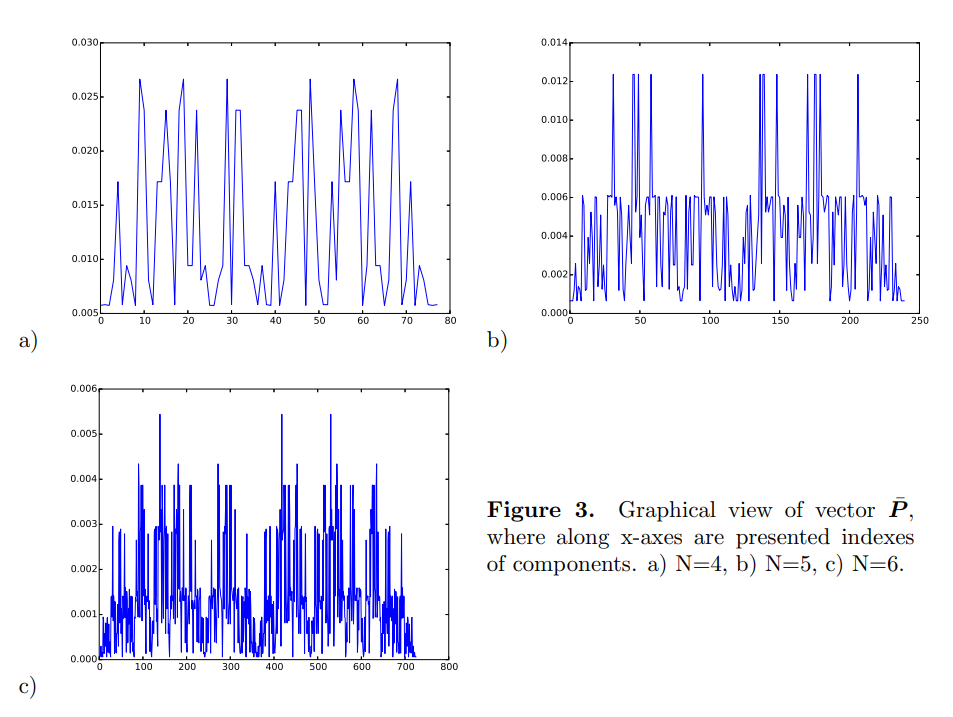
\includegraphics[width=0.7\textwidth]{Fig3.png}
\caption{Пример компонент стационарного вектора для $N=4$.}
\label{fig:3}
\end{figure}

\section{Реализация троичного генератора}

Стандартная реализация генератора представлена на рис. 4. Линия тактовых импульсов обозначает серию импульсов с интервалом $D$. Необходимо выбрать $D$ таким, чтобы времени было достаточно для перехода ГИСЧ в устойчивое состояние. В реальной ситуации невозможно получить стационарное распределение за конечное время; поэтому можно достичь лишь приближения к стационарному распределению.

\begin{figure}[h]
\centering
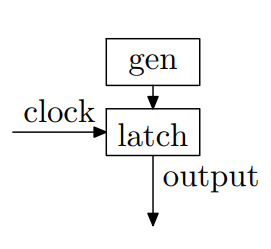
\includegraphics[width=0.5\textwidth]{Fig4.png}
\caption{Реализация. Здесь gen — ГИСЧ, выходы которого управляются тактовым сигналом.}
\label{fig:4}
\end{figure}

Малая нестабильность $D$ не влияет на это распределение. Для этого мы должны оценить разницу между устойчивой матрицей $Stab$ размера $M' \times M'$ вида
\[
Stab = (\overline{\mathbf{P}}, \overline{\mathbf{P}}, \ldots, \overline{\mathbf{P}})
\]
и матрицей $Astab(D) = \exp(D \cdot Matr)$. Пусть $\mathbf{E} = \langle 1,1,1,\ldots,1 \rangle$. Согласно определению, $\mathbf{E} \cdot Matr = \Theta = \langle 0,0,\ldots,0 \rangle$; следовательно, $\mathbf{E} \cdot Matr^k = \Theta$ для любого натурального $k$, и $\mathbf{E} \cdot Astab(D) = \mathbf{E}$. Другими словами, сумма элементов в любом столбце $Astab(D)$ равна 1. Пусть
\begin{equation}
\delta = \max_{k} |\overline{\mathbf{P}} - Astab(D)[*,k]|, \tag{12}
\end{equation}
где для вектора $\mathbf{q} = \langle a_1, \ldots, a_n \rangle$ $|\mathbf{q}| = \max_k |a_k|$. Выберем $\delta$ в качестве расстояния между двумя матрицами. Некоторые результаты вычислений представлены в таблице 2.

\begin{table}[h]
\centering
\caption{Расстояние между устойчивой матрицей и $Astab(D)$ в зависимости от $D$.}
\label{tab:2}
\begin{tabular}{c|cccc}
$N$ \ $D$ & 2 & 4 & 8 & 16 \\ \hline
1 & 3.1e-2 & 1.6e-3 & 3.9e-6 & 2.1e-7 \\
2 & 4.6e-2 & 6.1e-3 & 1.1e-4 & 3.8e-8 \\
3 & 3.6e-2 & 6.9e-3 & 2.4e-4 & 3.2e-7 \\
4 & 2.1e-2 & 3.7e-3 & 1.4e-4 & 2.6e-7 \\
5 & 9.8e-3 & 2.1e-3 & 9.2e-5 & 2.0e-7 \\
6 & 6.0e-3 & 9.4e-4 & 3.6e-5 & 7.1e-8
\end{tabular}
\end{table}

Как упоминалось выше, недостатком предложенного ГИСЧ является отсутствие трёх специальных сигналов вида $\langle x, x, \ldots, x \rangle$, $x \in \{-1,0,1\}$, которые не выдаются на выходах схемы. Можно предложить два метода преодоления этого недостатка. Первый — использование набора независимых ГИСЧ (рис. 5). Эта схема выдаёт равномерно распределённые сигналы.

\begin{figure}[h]
\centering
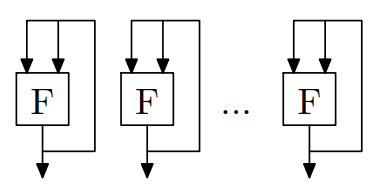
\includegraphics[width=0.5\textwidth]{Fig5.png}
\caption{Генератор на основе независимых элементов.}
\label{fig:5}
\end{figure}

На рис. 5 каждый ГИСЧ содержит один элемент, но можно использовать ГИСЧ с произвольным числом элементов в такой реализации, хотя в этом случае будет использоваться выход только одного элемента.

Существует другое решение проблемы отсутствия трёх особых состояний на выходах ГИСЧ. Предположим, у нас есть схема, представленная на рис. 6. Выход элемента 0 опущен. Из-за циклической структуры ГИСЧ можно опустить любой выход, но распределение выходных сигналов будет одинаковым. В результате на выходах ГИСЧ может возникнуть любой троичный вектор, и распределение этих векторов можно найти на основе предыдущих вычислений. Например, для $N=3$, если используются только два выхода, получаем вероятности (см. (11)):
\begin{itemize}
\item состояния $\langle x,x \rangle$ — 0.074;
\item состояния $\langle 0,1 \rangle$, $\langle -1,0 \rangle$, $\langle 1,-1 \rangle$ — 0.148;
\item все остальные состояния — 0.111.
\end{itemize}
Таким образом, распределение состояний становится немного ближе к равномерному, чем в исходном примере.

\begin{figure}[h]
\centering
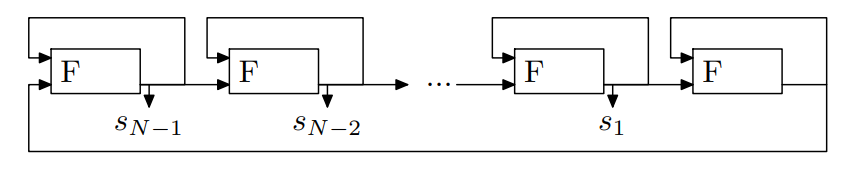
\includegraphics[width=0.4\textwidth]{Fig6.png}
\caption{Генератор с опущенным выходом.}
\label{fig:6}
\end{figure}

\section{Заключение}

Предположение о том, что времена задержки в различных элементах являются независимыми событиями, является естественным, в то время как ограничение на вид распределения является гораздо более сильным. В силу симметрии схемы, если время задержки для всех элементов имеет одинаковое распределение, то выход каждого элемента будет равномерным независимо от распределения. Тем не менее, существование стационарного распределения и его вид, если оно существует, требуют дополнительных исследований.

\section*{Приложения}

\subsection*{Доказательство предложения 1}

Пусть $F(a,b)$ удовлетворяет (2) и $F(0,0) = c_1$, $F(1,1) = c_2$, $F(-1,-1) = c_3$. Имеются следующие альтернативы:
\begin{enumerate}
\item $c_1, c_2, c_3$ — перестановка $0,1,-1$;
\item ровно два элемента в множестве $c_1, c_2, c_3$ равны.
\end{enumerate}

Рассмотрим первый случай. Пусть $c_1 = 1$. Поскольку все $c_i$ различны и $c_3 \neq -1$, имеем $c_3 = 0$. Тогда $F = F_1$. Если $c_1 = -1$, то $c_2 = 0$ и $c_3 = 1$. Используя перестановку $\sigma(0) = 0, \sigma(1) = -1, \sigma(-1) = 1$, преобразуем $F$ к $F_1$.

Теперь рассмотрим второй случай. Рассмотрим различные возможные распределения значений для $c_1, c_2, c_3$:
\begin{itemize}
\item $c_1 = 1, c_2 = 0, c_3 = 1$. Перестановка $\sigma(0) = -1, \sigma(1) = 1, \sigma(-1) = 0$ преобразует $F$ к $F_2$.
\item $c_1 = 1, c_2 = 0, c_3 = 0$. Перестановка $\sigma(0) = 1, \sigma(1) = -1, \sigma(-1) = 0$ преобразует $F$ к $F_2$.
\end{itemize}
Если $c_1 = -1$, то перестановка $\sigma(0) = 0, \sigma(1) = -1, \sigma(-1) = 1$ сводит дело к предыдущей ситуации.

\subsection*{Доказательство предложения 2}

Прежде всего, покажем, что $\mathbf{S} = \langle x, x, \ldots, x \rangle$ является недостижимым состоянием. Поскольку во время перехода может измениться только один выход, любое состояние-кандидат для перехода в $S$ должно иметь вид $\langle x, x, \ldots, x, y, \ldots, x \rangle$. Любой элемент в схеме имеет на входах либо $\langle x, x \rangle$, либо $\langle x, y \rangle$, либо $\langle y, x \rangle$. Во всех этих случаях элемент может изменить свой выход на $x$ в соответствии с определением $F$. С другой стороны, если $\mathbf{S} = \langle \ldots, x, y, \ldots \rangle$, где $x \neq y$, то состояние $\langle \ldots, x, z, \ldots \rangle$, где $z \neq x$ и $z \neq y$, может перейти в $\mathbf{S}$.

\subsection*{Доказательство предложения 3}

Согласно определению, элемент $Q[i,j]$ в строке с номером $i$ и столбце с номером $j$ равен 1 тогда и только тогда, когда генератор может перейти из состояния с номером $j$ в состояние с номером $i$. Поскольку генератор имеет $N$ элементов, каждый из них может изменить свой выход, и все новые состояния различны. Отсюда следует, что для каждого $j$
\begin{equation}
\sum_i Q[i,j] = N. \tag{13}
\end{equation}
Это означает, что $Q^T / N$ является стохастической матрицей, следовательно, $e_1 = N$, и выполняется неравенство (8).

\begin{thebibliography}{99}
\bibitem{1} Asmussen S and Glynn P W 2007 \textit{Stochastic Simulation: Algorithms and Analysis} (New York: Springer Verlag) p 476
\bibitem{2} Ferguson N, Schneie B, and Kohno T 2010 \textit{Cryptography Engineering: Design Principles and Practical Applications} (Indianapolis: Wiley) p 384
\bibitem{3} Horowitz P and Hill W 1980 \textit{The art of electronics} (Cambridge: Cambridge University Press) p 1125
\bibitem{4} Petrie C S and Connelly J A 1996 A noise-based IC random number generator for applications in cryptography \textit{Proc. IEEE Int. Symp. Circuits and Systems} (Atlanta) vol 4 (New York: IEEE Press) pp 324--327
\bibitem{5} Golic J D 2006 New Methods for Digital Generation and Postprocessing of Random Data \textit{IEEE Trans. Comput.} \textbf{55} 1217--1229
\bibitem{6} Sunar B, Martin W J and Stinson D R 2007 A provably secure true random number generator with built-in tolerance to active attacks \textit{IEEE Trans. Comput.} \textbf{56} 109--119
\bibitem{7} Kuznetsov V, Pesoshin V and Stolov E 2008 Markov model of a digital stochastic generator \textit{Automation and Remote Control} \textbf{69} 1504--1509
\bibitem{8} Wieczorek P and Golofit K 2014 Dual-Metastability Time-Competitive True Random Number Generator \textit{IEEE Trans. Circuits and Systems} \textbf{61} 134--145
\bibitem{9} Wu X W and Prosser F P 1990 CMOS ternary logic circuits \textit{IEE Proc. Circuits, Devices and Systems} \textbf{137} 21--27
\bibitem{10} Gaikwad V N and Deshmukh P R 2015 Design of CMOS ternary logic family based on single supply voltage \textit{Proc. IEEE Int. Conf. on Pervasive Computing} (Sydney) vol 9 (New York: IEEE Press) pp 1--6
\bibitem{11} Lisa N J and Babu H H 2015 Design of a Compact Ternary Parallel Adder/Subtractor Circuit in Quantum Computing \textit{Proc. IEEE Int. Symp. on Circuits and Systems} (Lisbon) vol 28 (New York: IEEE Press) pp 2145--2148
\bibitem{12} Kleinrock L 1975 \textit{Queueing Systems: Volume I Theory} (New York: Wiley-Interscience) p 417
\bibitem{13} Marcus M and Mink H 1964 \textit{A survey of matrix theory and matrix inequalities} (Boston: Allys and Bacon) p 232
\bibitem{14} Bellman R 1960 \textit{Introduction to matrix analysis} (New York: Macgrow-Hill) p 365
\end{thebibliography}

\end{document}